\section{Hiperparámetro \emph{reward}} \label{anexo:hyperReward}

El hiperparámetro \emph{reward} define qué función de recompensa se usará durante el entrenamiento. Hay dos opciones (ver tabla \ref{tab:rewardParameters}) que se nombran igual que la implementación de sus correspondientes clases en el código.

\begin{table}[h]
    \centering
    \begin{tabular}{lr}
        \toprule
        Clase            & Número de experimentos \\
        \midrule
        RewardFunction01 & 123                    \\
        RewardFunction02 & 28                     \\
        \bottomrule
    \end{tabular}
    \caption{Número de experimentos realizados para cada clase de función de recompensa}
    \label{tab:rewardParameters}
\end{table}

Estas funciones comparten la siguiente recompensa terminal:

$$
    R_T^1 =
    \begin{cases}
        +1000, & \text{el jugador 1 gana},   \\
        -1000, & \text{el jugador 1 pierde}.
    \end{cases}
$$

Lo que diferencia a estas funciones es la recompensa de los turnos intermedios, tal como se explica a continuación:

\begin{itemize}
    \item \textbf{RewardFunction01}: cada turno intermedio que el jugador continua en la batalla, es recompensado con $+1$.

    \item \textbf{RewardFunction02}: para ambos jugadores, el porcentaje de vida restante de todos sus Pokémon ($\mathsf{HP}$) siempre es conocido. Es posible tener en cuenta la diferencia de vida entre dos turnos consecutivos y usar esta diferencia como recompensa. Un incremento en la vida de un Pokémon propio es una acción positiva, mientras que una reducción en la vida de un Pokémon propio es una acción negativa. Lógicamente (es un problema de suma cero), ocurre lo contrario con la vida del oponente.

          Un ejemplo de esto se puede ver en la ilustración \ref{fig:turn6}, que muestra un turno de una batalla un Pokémon \emph{Grafaiai} propio y un Pokémon \emph{Mightyena} del oponente. El \emph{Grafaiai} propio le inflinge 11\% de daño al \emph{Mightyena}, mientras que \emph{Mightyena} le ocasiona 31\% de daño a \emph{Grafaiai}. La recompensa para el jugador propio será entonces $-0.31 - (-0.11) = -0.2$.

          \begin{figure}[h]
              \centering
              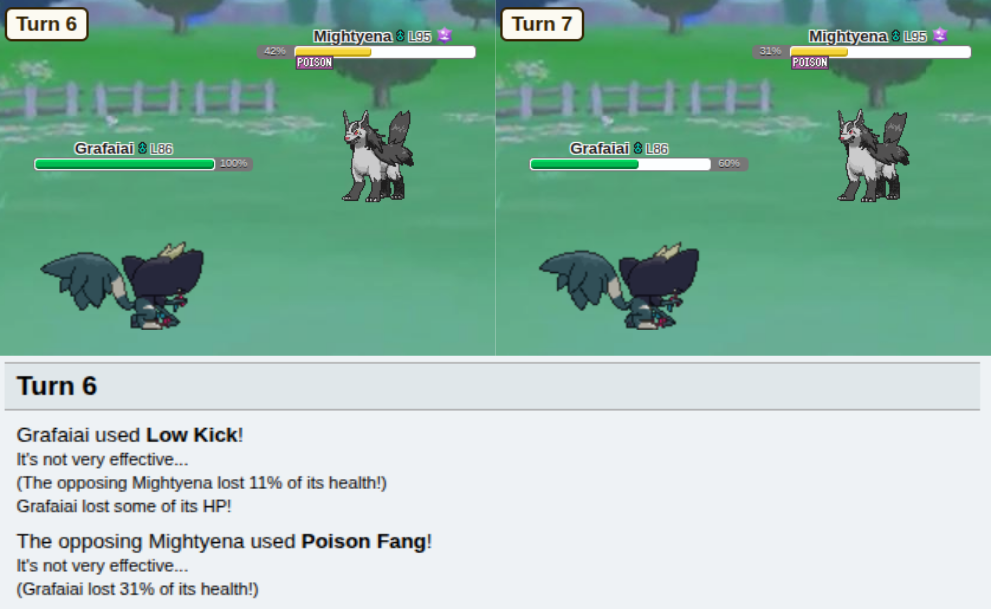
\includegraphics[width=0.8\textwidth]{images/turn6.png}
              \caption{Turno de un combate Pokémon que ejemplifica la función de recompensa \emph{RewardFunction02}}
              \label{fig:turn6}
          \end{figure}
\end{itemize}
